\documentclass{book}
\usepackage{amsmath}

\usepackage{mathtools}
\usepackage{algpseudocode}
\usepackage{algorithm} 
\usepackage{bm}
\usepackage{graphicx}
\usepackage{setspace}

\usepackage[round]{natbib}
\usepackage{tikz}
\usepackage{tikz-qtree}
\usepackage{tikz-dependency}

\usepackage[left=1in, right=1in, top=1in, bottom=1in]{geometry}

\title{Parsing}

\begin{document}


%\chapter*{\centering \begin{normalsize}Abstract\end{normalsize}}
\chapter*{\centering Abstract}
\begin{quotation}
\noindent % abstract text
\end{quotation}

In this thesis, we describe about the state of the art probabilistic unsupervised dependency parser, Dependency Model with Valence (DMV) \citep{klein2004}. It induces dependency trees from parts-of-speech tag sequences. DMV uses ad-harmonic initializer. As an extension, we experiment using several hundred random restarts of the EM instead of ad-harmonic initializer. The highest undirected accuracy and directed accuracy achieved by random initializations were 70.56\% and 55.59\% respectively. These were 5\% and 4\% greater than the original implementation using just ad-harmonic initializer.


\let\cleardoublepage\clearpage

\chapter{Introduction}


Parsing is one of the fundamental areas in natural language processing. A sentence can have many possible syntactic trees. The parser builds a model which scores each of these trees and outputs the one with the highest score. Thus, parsing is mapping a sentence to a predicted structure.

\section{Dependency and Constituency}

In natural language processing, two linguistic structures are widely known: phrase structure trees and dependency trees.

  In linguistics, phrase structure grammars are those that are based on the constituency relation. The non-leaf nodes of the phrase structure tree consist of non-terminal symbols representing particular constituent phrases. In the example given below, the noun phrase (NP) and the verb phrase (VP) are the constituents. The leaves are the terminal symbols representing the individual words.

A dependency tree of a sentence is a directed acyclic graph rooted at the special symbol ROOT. The tree has to be projective, that is no two edges can cross each other. It is comprised of a series of dependencies. A dependency is an ordered pair of (head, modifier) words. Every word but for the ROOT can have only one head word in all. The ROOT of the whole parse can never be a modifier. The directed edge is drawn from the head word to the modifier.

\begin{figure}
\centering
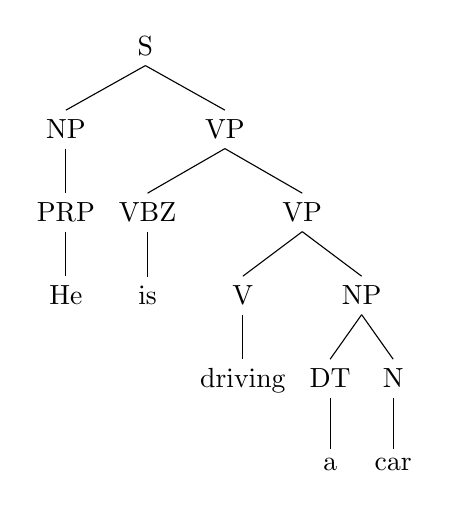
\begin{tikzpicture}

\Tree 
[.{S}
    [.{NP}
        [.{PRP}
          [.{He} ] 
        ] 
    ]
    [.{VP} 
        [.{VBZ}  
          [.{is}  ]
        ] 
        [.{VP} 
          [.{V} 
            [.{driving}  ]
          ]
          [.{NP} 
            [.{DT} 
              [.{a}  ]
            ]
            [.{N} 
              [.{car}  ]
            ]
          ] 
        ]
    ]
]
\end{tikzpicture}

\begin{dependency}[theme = simple]
\begin{deptext}
root \& He \& is \& driving \& a \& car \\
\end{deptext}
\depedge{1}{4}{}
\depedge{4}{3}{}
\depedge{4}{2}{}
\depedge{4}{6}{}
\depedge{6}{5}{}
\end{dependency}
\caption{Phrase Structure Tree and Dependency Tree for the sentence ``He is driving a car''}
\end{figure}

The time complexity to parse phrase structure grammar using CKY $O(n^3G^3)$ where G is the number of non-terminals in the grammar. The time taken to parse a lexicalized phrase structure grammar, where the non-terminals include the head word of the constituent, is $O(n^5G^3)$. As opposed to this, the dependency grammar can be parsed in $O(n^3)$. As it can be observed in the diagram, the phrase structure trees take up also a lot of memory in comparison to the dependency trees, to store the additional non terminals. Thus, the use of dependency trees has been on the rise in NLP. 

\section{Why build parsers}

Parsing has several applications. 

\begin{enumerate}

\item It is used to check the grammatical correctness of a sentence. If the sentence complies with the grammar devised by the parser, then it is grammatically correct.

\item It determines how probable a sentence is. This is very useful in the case of natural language generation. For example, we could compare the scores of the parse trees for the sentences ``I am flying an airplane'' and ``An airplane I am flying'' , and deduce which sentence is more probable.

\item It is also used as an intermediate stage in semantic analysis for question answering and relationship extraction. Given a sentence ``Ban ki moon is the general secretary of the United Nations.'', we could query the computer ``who is the general secretary of the United Nations$?$''. It would look up the NP constituent of the phrase structure tree and reply ``Ban ki Moon.''



\begin{figure}
\centering
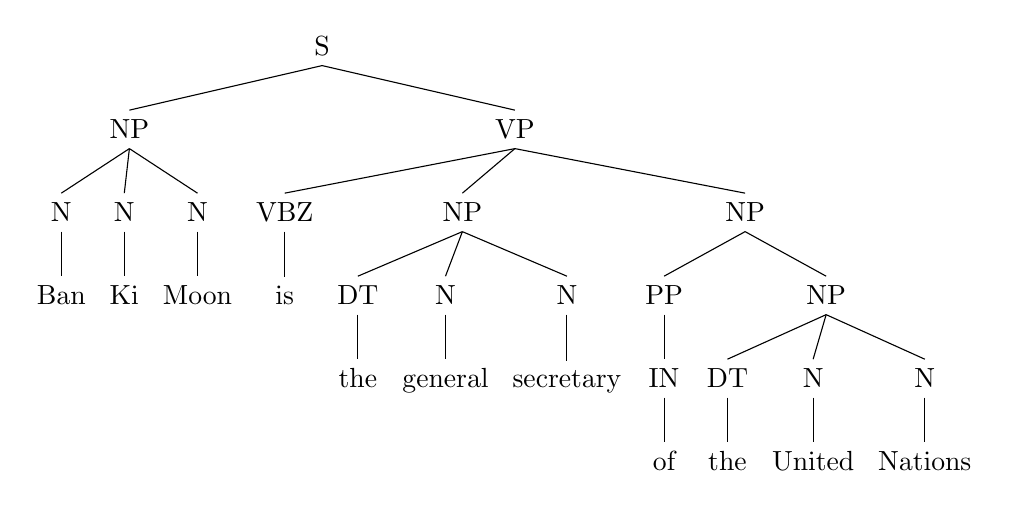
\begin{tikzpicture}

\Tree 
[.{S}
    [.{NP}
        [.{N}
          [.{Ban} ] 
        ] 
        [.{N}
          [.{Ki} ] 
        ] 
        [.{N}
          [.{Moon} ] 
        ] 
    ]
    [.{VP} 
        [.{VBZ}  
          [.{is}  ]
        ] 
        [.{NP} 
          [.{DT} 
            [.{the}  ]
          ]
          [.{N} 
            [.{general}  ]
          ]
          [.{N} 
            [.{secretary}  ]
          ]
        ] 
        [.{NP}
          [.{PP}
            [.{IN}
              [.{of}   ]
            ]
          ]
          [.{NP}
            [.{DT}
              [.{the}   ]
            ]
            [.{N}
              [.{United}   ]
            ]
            [.{N}
              [.{Nations}   ]
            ]
          ]  
        ]
    ]
]
\end{tikzpicture}
\caption{PST for the sentence ``Ban Ki Moon is the general secretary of the United Nations''}
\end{figure}


\item Parsing is the basis for syntactic machine translation. In English, all the sentences are of the form Subject Verb Object. While for most Asian Languages, they are of the form Subject Object Verb. So on translating a sentence from Hindi to English,

Translated from Hindi: She school goes to.

English : She goes to school.

We could correctly translate by swapping the verb and object from the generated tree.



\end{enumerate}

\section{Motivation for Unsupervised parsing}

A \textit{manually annotated dependency treebank} is comprised of a large number of sentences and their corresponding human-annotated dependency trees. The dependency tree for each sentence is manually built by linguists using a common annotation manual. When a parser learns from manually annotated training data, it is called \textit{supervised parsing}. When a parser builds a model from unannotated data, it is called \textit{unsupervised parsing}. It relies heavily on the redundancy of the patterns in the data.

Building manually annotated treebanks is time consuming and expensive. Human annotators are also prone to errors. Not all languages have annotated treebanks. The linguists annotating the treebanks might differ about what the correct dependency tree is. Also, different treebanks might differ in the underlying linguistic formalisms and data formats. The labels for the part-of-speech tags, constituents, and dependencies might vary drastically. Owing to this, the linguistic tools working on one treebank cannot be easily extended to other languages simply by adding new treebanks. An experiment on harmonizing all the available treebanks \citep{zeman2012} showed that automatic transformation between different annotation styles cannot be lossless, as various kinds of linguistic information expressed in one annotation style often cannot be captured in another style.

Another problem with treebanks is that they are domain dependent. For example, the English Penn Treebank \citep{marcus1994} consists of newspaper articles. Parsers trained on Penn Treebank achieve very good results on held-out data from the very same domain, but on using them to parse books, their accuracy deteriorates. 

The linguistic rules cannot be incorporated for unsupervised parsing.  We define the linguistic assumptions allowed for unsupervised parsing as those that are independent of language and tag set.

The output of unsupervised parsers, despite having low accuracy, could be used as a first parse for annotating large treebanks \citep{vanzaanen2000}. They could also be used in systems like named-entity detectors that incorporate the parse features but do not require them to be perfect.


\section{History of unsupervised grammar induction}

One of the main goals of researchers since the advent of computational linguistics is to induce grammar from raw text. They started off with computing mutual information between words in the text. \citep{vander1978} \citep{magerman1990}

\citep{carroll1992} learnt about the syntactic structure of a language from examples of sentences in the language that have not been (fully) annotated . They split the data into two parts. From the first part, they extracted the rules that generate that part of the text and computed the initial probability. They ran the EM algorithm on the second part to compute the final probabilities. However, the quality of the induced grammar was very poor. On enforcing some constraints on the rules, they were able to improve the quality of the grammar induced. 

\citep{yuret1998} experimented with mutual independence of edges. The probability of a dependency tree is computed as a product over all nodes’ conditional on their parents. Maximizing such a product is equal to maximizing the product of the point-wise mutual information between parent and child for individual dependency edges. \citep{paskin2002} suggested a stronger assumption that all children (dependents) of a particular word are mutually independent and that their relative ordering is independent of their parent word. The dependency tree is a combination of the depedency structure $D$ (Figure 2.1) and the words $w$ over which this structure is built. According to Paskin's model, to generate a dependency tree, the dependency structure is generated uniformly and then the words are filled in. The probabilistic model is: 

\begin{gather*}
P(D) = P(s,G) \\ 
     = P(G)P(S|G)\\
     = P(G) \prod_{(i,j,dir) \in G} P(_{i-1}s_{i}|_{j-1}s_{j},dir)
\end{gather*}


\begin{figure}[!ht]
\centering
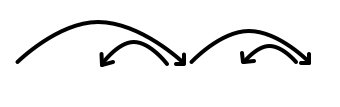
\includegraphics[width=90mm]{images/dep_structure.jpg}
\caption{Dependency Structure}
\label{overflow}
\end{figure}


Neither of these approaches yielded satisfactory results.

\citep{klein2004} proposed that conditioning the generation of a dependent only on its parent is not enough. They introduced the notion of valence to the dependency model. The term valence is used in similar context as it is used in chemistry. In chemistry, valency refers to the number of free electrons available in an atom to form a bond. In their model, valence refers to whether the dependent is the first child of the head word or not. They realized that adding too much information such as if it is the first, second or nth dependent was dangerous.

\section{Dependency Model with Valence}

Dependency Model with Valence (DMV) is an unsupervised model of dependency parsing which has the following steps:

\begin{itemize}

\item First, the root of the sentence is generated and it further generates its dependents.

\item For each node, all the right dependents are generated to begin with. After all the dependents are generated on the right, a STOP symbol is generated. This STOP symbol indicates that the current word no longer takes any arguments in the present direction. This is followed by the generation of all the left dependents and a STOP symbol on the left. 

\item Every time before a dependent is generated in a particular direction, a decision is made if the STOP symbol should be generated or it should continue generating dependents. The probability of generating a STOP symbol next is conditioned on the identity of the head and the direction of the attachment and the adjacency (adj) $P_{STOP}(\neg STOP | h, dir, adj)$. Adjacency indicates whether or not a dependent is the first modifier of the head word in the current direction.

\item A head word takes a dependent in a particular direction conditioned on the head word itself and the direction in which the dependent is taken $P_{CHOOSE}(a|h, dir)$. This entire process is recursive.

\end{itemize}

For a dependency structure $D$, let each word $h$ have left dependents $deps_D(h, l)$ and right dependents $deps_D(h, r)$. The probability of the fragment $D(h)$ of the dependency tree rooted at $h$ is given by:

\begin{gather*}
    P(D(h)) = \prod\limits_{dir\in(l,r)} \prod\limits_{a\in deps_D(h,dir)} P_{STOP} (\neg STOP | h, dir, adj) \\
    P_{CHOOSE}(a|h, dir) P(D(a)) P_{STOP}(STOP | h, dir, adj)
\end{gather*}

The DMV can be expressed as a lexicalized PCFG. The rules of the grammar are given in table 1.1:


\begin{table}[htbp]
\onehalfspacing
\begin{center}
\begin{tabular}{|c|}
 \hline
  Head choice (right-first)   $\overrightarrow{w}$  $\rightarrow$ w \\
  Head choice (left-first)   $\overleftarrow{w}$   $\rightarrow$ w \\

  Right-first right attachment $\overrightarrow{h}$  $\rightarrow$ $\overrightarrow{h}$ a \\
  Right-first right stop $\overleftarrow{\overrightarrow{h}}$ $\rightarrow$ $\overrightarrow{h}$ \\
  Right-first left attachment $\overleftarrow{\overrightarrow{h}}$ $\rightarrow$ a $\overrightarrow{h}$ \\
  Right-first seal $\bar{h}$ $\rightarrow$ $\overleftarrow{\overrightarrow{h}}$ \\

  Left-first left attachment  $\overleftarrow{h}$ $\rightarrow$  a $\overleftarrow{h}$ \\
  Left-first left stop  $\overrightarrow{\overleftarrow{h}}$ $\rightarrow$ $\overleftarrow{h}$ \\
  Left-first right attachment $\overrightarrow{\overleftarrow{h}}$ $\rightarrow$ $\overrightarrow{\overleftarrow{h}}$ a \\
  Left-first seal $\bar{h}$ $\rightarrow$ $\overrightarrow{\overleftarrow{h}}$ \\
 \hline
\end{tabular}
\end{center}
\caption{Rules of the PCFG For DMV}
\end{table}

\begin{figure}[!ht]
\centering
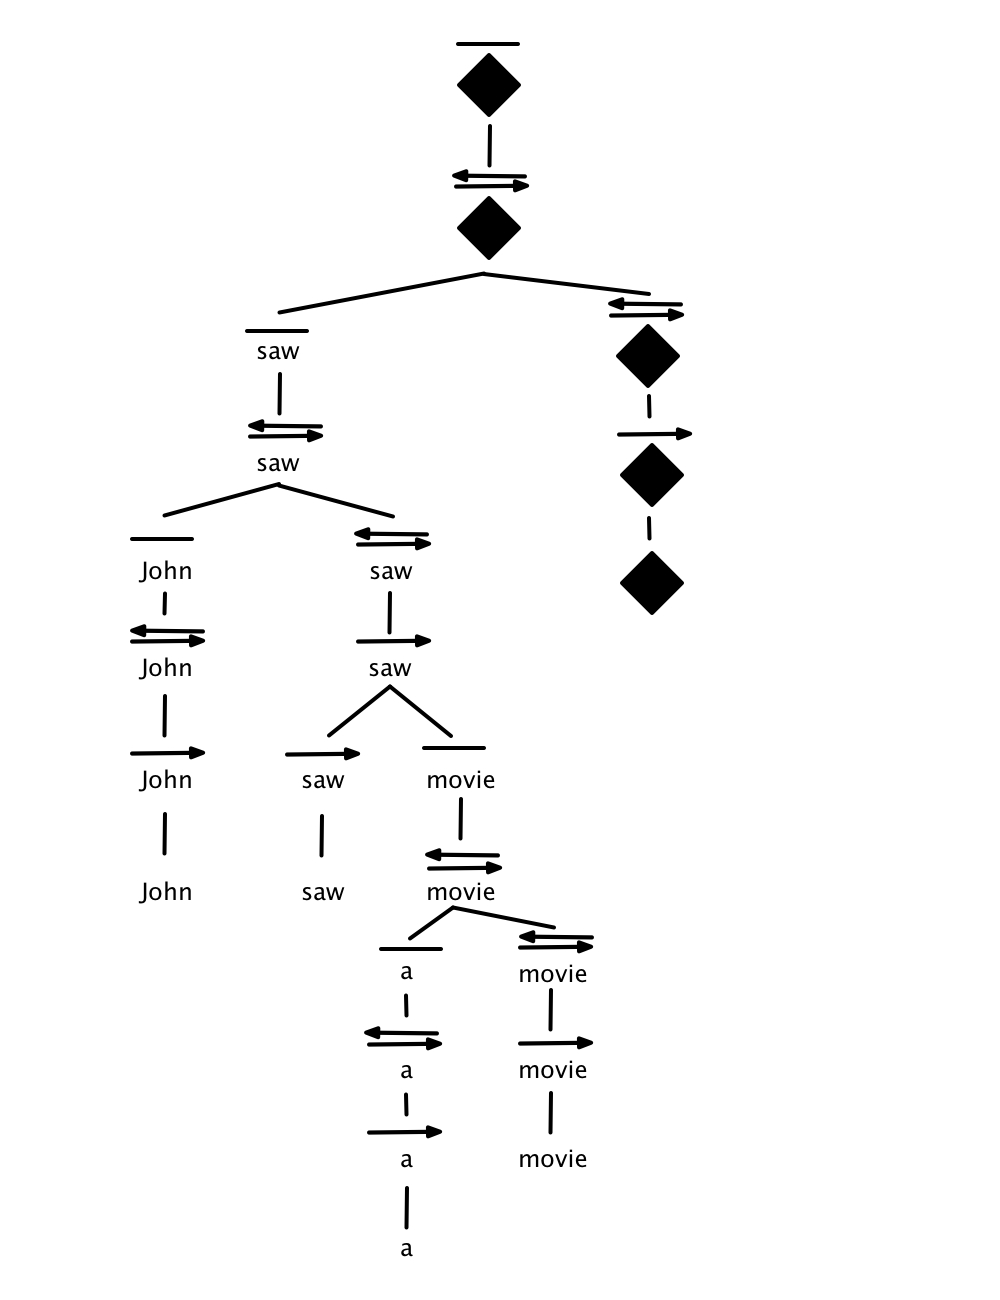
\includegraphics[width=90mm]{images/DMV_grammar.jpg}
\caption{A tree formed using the rules for DMV for the sentence ``John saw a movie''}
\label{overflow}
\end{figure}

\section{Existing variants of DMV}

\citep{smith2005} used contrastive estimation together with DMV. The learner is given some positive examples and negative examples. These negative examples are slight perturbations of the positive examples and are semantically close to them. But they are grammatically incorrect. When running the EM algorithm, the local neighbourhood is a set of implicit negative examples along with one positive example. Thus the local maxima is always the positive example. A learner is said to build a good model if it is able to discriminate the positive sentence from the neighbourhood. The goal of CE is to move the probability mass from the neighbouring sentences to the positive sentence.

\citep{cohen2008} used logistic normal priors to encode information about which grammar rules are likely to vary. They are more intuitive and expressive representation of the knowledge than Dirichlet distributions. These priors encourage sparse solutions, a property which is important for grammar induction. They derived a variational EM algorithm for the probability estimation and achieved a 59.4\% directed attachment score on WSJ10. 

\citep{headden2009} extended the valence and conditioned generating a new argument on whether it is adjacent or not. The probability $P_{CHOOSE}(a|h, dir)$ in the above equation is thus substituted by $P_{CHOOSE}(a|h, dir, adj)$. He called it Extended Valence Grammar (EVG). Headden et al. also used the lexicalization (the generated arguments are conditioned not only the head part-of-speech but also its word form) and smoothing by interpolation increasing the directed attachment score to 68.9\%.
$$P_{ATTACH}(a|h,dir,adj) = \lambda_1P_1(a|h,dir,adj) + \lambda_2P_2(a|dir,adj)$$

where $\lambda_1$ and $\lambda_2$ sum up to 1.
   
\citep{spitkovsky2011b} observed a strong connection between English punctuation and phrase boundaries, split sentences at punctuation marks and imposed parsing restrictions over their fragments.

\section{Initialization of DMV}

The Expectation Maximization algorithm finds a local maximum of its objective function. Probabilistic dependency grammars have several local maxima. One of the most important factors in avoiding EM getting stuck in a local maxima is its initialization. DMV uses an \textbf{ad-harmonic initializer}. 

Consider a sentence with words $w_1$ $\ldots$ $w_n$ where $n$ is the number of words in the sentence.\\

(1) Each word has a uniform probability of becoming a ROOT.

   $$ P(ROOT) =  \frac{1}{n} $$

(2) The probability of dependency between two words is inversely proportional to the distance between them.

\begin{align*}
  \forall{i,j},  \;\, 1 \le j \le n \; total[w_j] &= \sum_{1 \le i \le n \, and \, i \ne j} \frac{1}{|{j-i}|} \\
   \forall{i,j},  \;\, j < i \le n \; P(w_i| w_j, right)  &= \frac{(n-1)}{n} \times \frac{1}{total[w_j]} \times \frac{1}{|{j-i}|} \\
    \forall{i,j}, \;\, i < j \le n \; P(w_i| w_j, left)  &=  \frac{(n-1)}{n} \times \frac{1}{total[w_j]} \times \frac{1}{|{j-i}|}
\end{align*}

The initializer is built under the linguistic intuition that shorter dependencies are preferable to longer. Many techniques have been conceived to help EM achieve better likelihood, two of which that are relevant to us are discussed in this section.

\citep{smith2006} proposed ``The Skewed Deterministic Annealing and Structural Annealing techniques'' where the initial parameter settings are biased to reflect this intuition that short dependencies are better. This bias is slowly removed over the course of learning. Deterministic Annealing leads to flatter likelihood surface. This eventually helps in finding maxima with higher likelihood.

\citep{headden2009} used 100 instances of estimating DMV using using Variational Bayes, where each instance is given 20 random restarts. Each restart was run for 40 iterations, and the model with the highest lower bound value was run until convergence. His results indicate that directed accuracy of DMV using Variational Bayes with random initialization has increased by 6\% and undirected accuracy increased by 2\%.

\section{Goal of this Thesis}

 In order to overcome the problem of local maxima, we intend to use several hundred random restarts for DMV. The parameters for the random restart are generated by drawing values uniformly at random from the interval [0,1] and then normalizing.  We would like to observe the relationship between the likelihood of the objective function and the accuracy of the parser in each case. These models are then compared with the one produced by initializing the EM with the ad-harmonic initializer.

\chapter{Implementation}
A dependency parse is comprised of many (head word, modifier word) pairs. The modifier is dependent on the head word. Given a sentence, there are several such parses possible.

\begin{figure}[!ht]
\centering
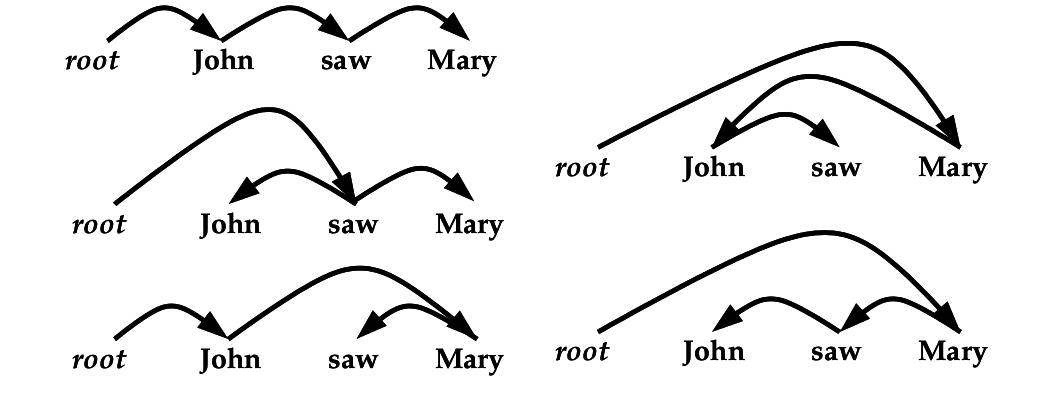
\includegraphics[width=90mm]{images/rsz_all_deps.jpg}
\caption{All possible parses for the sentence ``John saw Mary''}
\label{overflow}
\end{figure}


 Let $D$ be the set of all valid parses possible for a sentence. Every parse has a certain probability of being generated. Our goal is to identify the parse with the highest probability. Let counts() be a method that returns the number of times a particular parse occurred. The probability of a parse $S$ is computed as:

            $$P(S) = counts(S) / \sum_{t \in D} counts(t) $$

The motive of the parser is to obtain the parameters of the underlying distribution from which these sentences are produced. They are: 

\begin{itemize}
\item The probability that a head word takes a modifier (depProb[h, m, direction])
\item The probability that a head word continues to take further arguments (contProb[h, direction, adj])
\item The probability that a head word stops taking further arguments (stopProb[h, direction, adj]).
\end{itemize}


Eisner's parsing algorithm is used to keep track of the counts of all possible parses. A hypergraph is an efficient data structure that aids in calculating the probabilities of each one of these parses and the total probability of all the parses. Thus the crux of the implementation is building a hypergraph using all the possible parses.

\section{Eisner's parsing algorithm}

Here we discuss about a modified version of Eisner's parsing algorithm. The 3 basic components of this algorithm are: \textbf{incomplete constituents, complete constituents, complete stopped constituents}. Pictorially, they are represented by a trapezium, triangle and a triangle with a line respectively. The diagram given below illustrates how each one of them are formed. Any constituent has  3 attributes, namely, index of the head word, index of the modifier word and the direction. 

A complete constituent with head word h can choose to take another word as its dependent with a certain probability called the \textbf{continue probability}. The head word of a complete constituent stops taking further arguments in that direction with a probability called the \textbf{stop probability}, leading to the formation of a complete stopped constituent (rule 2). A word $h$ takes another word $m$ as its argument only after $m$ stopped taking arguments on both sides. Thus a complete constituent with head word $h$ combines with a complete stopped constituent $m$ to create an incomplete constituent (rule 1). An incomplete constituent with head word $h$ and modifier $m$ then combines with a complete stopped constituent whose head word is $m$ to form a complete constituent (rule 3). This continues until two complete stopped constituents are formed in either directions together spanning the entire sentence (Figure 2.3). A complete stopped constituent is a type of complete constituent. Every word by default is a complete constituent.

\begin{figure}
\centering
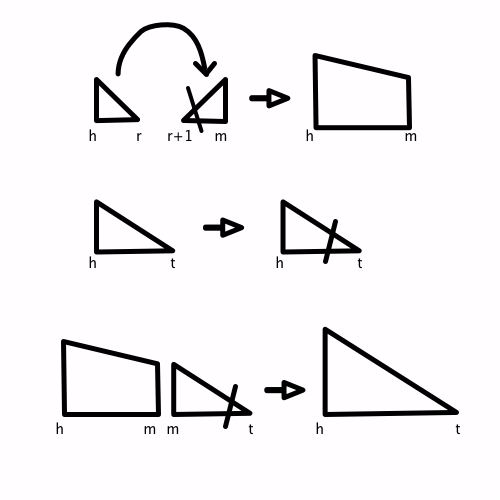
\includegraphics[width=90mm]{images/eisner_rules.jpg}
\caption{Eisner's algorithm rules}
\label{overflow}
\end{figure}


The pseuocode of Eisner's parsing is given in Algorithm 1. The dynamic programming table C[s][t][d][c] stores the sum of probabilities of the subtrees that can be formed from s to t in the direction d. c indicates the type of the constituent. if c = 0, it is an incomplete constituent. c = 1, it is a complete constituent. c = 2 indicates that it is a complete stop constituent.

Eisner's parsing algorithm is an efficient way to collect the counts for all the possible parses. The computational complexity of CKY algorithm for parsing lexicalized grammar is $\bm{O(n^5G^3)}$ while that of Eisner's algorithm is $\bm{O(n^3)}$.


\begin{algorithm}

\caption{Eisner's parsing algorithm}

\begin{algorithmic}

  \State Initialization:
     \For{s = 0 to n}

        \State \% Form complete constituent of size 1
        \State C[s][s][$\rightarrow$][1] = C[s][s][$\leftarrow$][1] = 0.0
        \State \% Form complete constituent stop of size 1
        \State C[s][s][$\rightarrow$][2] = C[s][s][$\rightarrow$][1] + S(s,s)
        \State C[s][s][$\leftarrow$][2] = C[s][s][$\leftarrow$][1] + S(s,s)

\EndFor


\For{ k = 1 to n + 1}
  \For{s = 0 to n}


    \State t=s+k
     \State if t $>$ n then break
     \State \% First: create incomplete constituent
      \State C[s][t][$\leftarrow$][0] = $\sum_{s \le r< t}$ (C[s][r][$\rightarrow$][2] + C[r + 1][t][$\leftarrow$][1] + S(t, s)) 
      \State C[s][t][$\rightarrow$][0] = $\sum_{s \le r<t}$ (C[s][r][$\rightarrow$][1] + C[r + 1][t][$\leftarrow$][2] + S(s, t)) 
      \State \% Second: create complete constituent
      \State C[s][t][$\leftarrow$][1] = $\sum_{s \le r<t}$ (C[s][r][$\leftarrow$][2] + C[r][t][$\leftarrow$][0])
      \State C[s][t][$\rightarrow$][1] = $\sum_{s<r \le t}$ (C[s][r][$\rightarrow$][0] + C[r][t][$\rightarrow$][2])
      \State \% Third: create complete constituent stop
      \State C[s][t][$\leftarrow$][2] = $\sum_{s \le r<t}$ (C[s][t][$\leftarrow$][1] + S(t,t))
      \State C[s][t][$\rightarrow$][2] = $\sum_{s<r \le t}$ (C[s][t][$\rightarrow$][1] + S(s,s))

\EndFor
\EndFor

      \State Return C[0][n][$\rightarrow$][2] as the highest score for any parse

\end{algorithmic}
\end{algorithm}


\begin{figure}
\centering
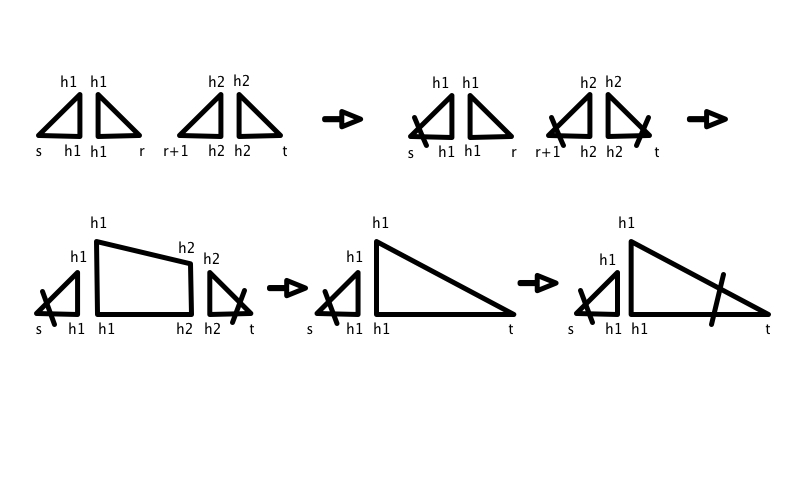
\includegraphics[width=90mm]{images/eisner_sentence.jpg}
\caption{Phases in Eisner's algorithm parsing a sentence}
\label{overflow}
\end{figure}

\section{Hypergraph}

A hypergraph is a pair H = $(V, E)$, where $V$ is the set of vertices, $E$ is the set of hyperedges. A weighted hypergraph is associated with the set of weights W. Each hyperedge $e$ $\in$ $E$ of a weighted graph is a triple $e~=~(T(e), h(e), f(e))$, where $h(e)$ $\in$ $V$ is its head vertex and $T(e)$ $\in$ $V^*$ is an ordered list of tail vertices. $f(e)$ is a weight function from $W|T(e)|$ to $W$.

The words in a sentence combine in different ways to form sub parses. The subparses form the vertices of the hypergraph. One or more of the sub parses that combine to generate another sub parse, form the tail nodes of the edge. The resultant subparse is the head node of the edge. 

\begin{figure}
\centering
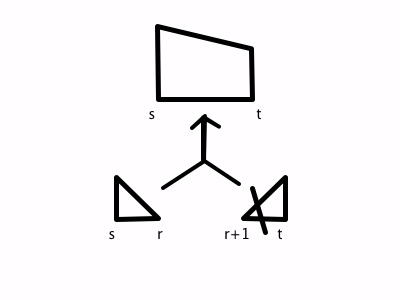
\includegraphics[width=90mm]{images/hypergraph_example.jpg}
\caption{A hypergraph}
\label{overflow}
\end{figure}


The weights of the edges are determined by an algorithm presented later. The best parse is the maximum weighted path encompassing all the words leading to the root. This is obtained by running viterbi algorithm on the entire hypergraph.
  The probability of a subparse SP formed at vertex $V_{SP}$, for a given sentence is given by:
            $$ P(V_{SP}) = \sum_{\forall e \in H(e) = V_{SP}} P(e) $$

The probability of this subparse for the entire grammar is obtained by summing P($V_{SP}$) for all the sentences in the corpus. These probabilities are used for calculating depCounts and stopCounts as given in the Algorithm section.

\section{Algorithm}

An open source library called PyDecode is used to build a hypergraph, with all the 3 constituents of the Eisner's parsing algorithm as its nodes. An edge has the head word, modifier word, direction, adjacency and state values stored in it. The direction indicates the direction in which the edge is being formed. The adjacency indicates if the modifier word is the first child of the head word, or not. If an edge does not have a modifier, the modifier word is `` ''.The edges of the hypergraph are assigned weights according to the algorithm 2:

\begin{algorithm}
\caption{Compute Weights}
\begin{algorithmic}


\State Lets assume incomplete constituent as i.c and complete constituent stop as c.s

\If{edge.headNode $\in$ i.c}
   \State return depProb[edge.headWord, edge.modifierWord, edge.dir] $\times$ contProb[edge.headWord, edge.dir, edge.isAdj]
\ElsIf{edge.headNode $\in$ c.s}
   \State return stopProb[edge.headWord, edge.dir, edge.isAdj]
\Else
   \State return 1
\EndIf

\end{algorithmic}
\end{algorithm}

 The insideOutside algorithm is run on the entire hypergraph. The inside probability of the root of the hypergraph gives the total probability of the sentence Z. The marginals of the nodes and the edges of the hypergraph are computed using the PyDecode library. marginals = marginals / Z gives the counts for the EM algorithm.

The em algorithm is run 10 times for all the sentences. The hypergraph is built for each sentence. The stop and dep probabilities are incremented according to Algorithm 3.


\begin{algorithm}
\caption{Update counts}
\begin{algorithmic}

\State Assume incomplete constituent to be i.c and complete constituent stop to be c.s

\For{edge in hypergraph.edges}

   \State headWord, modWord, direct, adj, state = edge.label.split()

       \If{edge.headNode $\in$ i.c}
          \State depCounts[headWord, modWord, direct, adj] += marginals[edge.label]
        \EndIf

        \If{edge.headNode $\in$ c.s}
          \State stopCounts[headWord, direct, adj] += marginals[edge.label]
        \EndIf

\EndFor

\end{algorithmic}
\end{algorithm}

\section{Maximum Likelihood Estimation}

The likelihood of a set of parameter values $\theta$, given outcome y, is the probability of the observed outcome given the parameter values. Maximum likelihood is the procedure of finding the value of one or more parameters for a given statistic which maximizes the known likelihood distribution.

Let $\overrightarrow{x}^t = (\overrightarrow{x_1^t}, \overrightarrow{x_2^t}, ..., \overrightarrow{x_{|x^t|}^t})$ be an unannotated training dataset. There are hidden dependency structures $y_i^t$ for each $x_i^t$. The DMV is a generative model. So it maximizes the joint probability of the input data and the hidden structures.


\begin{center}
$\overrightarrow{\theta}_{MLE} = \underset{\overrightarrow{\theta}}{argmax} P_{\overrightarrow{\theta}}(\overrightarrow{x}^t) = \underset{\overrightarrow{\theta}}{argmax} \sum\limits_{\overrightarrow{y}} P_{\overrightarrow{\theta}}(\overrightarrow{x}^t, \overrightarrow{y})$ \\
We assume all the sentences are sampled independently from the underlying distribution

$\overrightarrow{\theta}_{MLE} = \underset{\overrightarrow{\theta}}{argmax} \prod\limits_{i=1}^{|\overrightarrow{x}^t|} P_{\overrightarrow{\theta}}(\overrightarrow{x_{i}}^t) =
 \underset{\overrightarrow{\theta}}{argmax} \prod\limits_{i=1}^{|\overrightarrow{x}^t|} \sum\limits_{y \in Y_{x}} P_{\overrightarrow{\theta}}(\overrightarrow{x_{i}^t}, \overrightarrow{y})$

\end{center}

The maximum likelihood is estimated using the EM algorithm.

\section{EM}

\textbf{The expectation maximization (EM)} algorithm is used to estimate the parameters of models built using latent variables. One iteration of the EM algorithm is constituted of two steps : the Expectation step and the Maximization step. 

The \textbf{Expectation (E) step} uses the current parameters $\theta_t$ to construct a function l($\theta | \theta_t$). The function l($\theta | \theta_t$) is a lower bound to the true objective L($\theta$) and matches L($\theta$) exactly at $\theta_t$.

The \textbf{maximization (M) step}, which computes parameters maximizing the expected log-likelihood constructed in the E step.

These two steps are repeated until convergence. The characteristic of EM is that the likelihood always increases and is guaranteed to convergebut not to global optimum.

The EM formulated for a parser estimates the parameters of the grammar, namely the depProb, stopProb and contProb as mentioned in the introduction. It is run on all the sentences in the corpus for 10 iterations. The Wall Street Journal's sections 2 to 21 of the Penn Treebank were used as the corpus for building the model. For every sentence, the depCounts and stopCounts are incremented as illustrated in Algorithm 3. At the end of each iteration, the depProb, stopProb and contProb are re-estimated. After each iteration, EM algorithm gradually increases the probability of the events occuring more often and reduces that which are not.

\begin{itemize}

\item Let the vocabulary generated by the grammar be ${\cal W}$, the modifier word be $m$, head word be $h$ and the direction in which the head word takes the argument be be $dir$.
\item Let the type of incomplete constituent be $Trap$, complete constituent be $Tri$ and complete stop constituent be $TriStop$
\item Let edge $E$ = \{E.headWord $\in$ Trap, E.headWord $\in$ Tri, E.headWord $\in$ TriStop\}
\item The label of an edge consits of headWord h, modifier m, direction dir, CONT, ADJ as mentioned in the earlier section
\item We are given marginals $p(E)$

\end{itemize}

Algorithm 4 defines the EM algorithm for the parser.

\begin{algorithm}

\caption{EM algorithm for DMV}

\begin{algorithmic}

\For{iterations =1 to 10}
\State \# Estimation Step
   \For{sentence in corpus}

         \[stopCounts(h, dir, \mathrm{ADJ}= 1, CONT = 0) =
           \sum p(\mathrm{E(h, dir, ADJ=1, CONT = 0)}) \]

         \[stopCounts(h, dir, \mathrm{ADJ}= 1, CONT = 1) = 
           \sum p(\mathrm{E(h, dir, ADJ=1, CONT = 1)}) \]

         \[depCounts(h, m, dir) =
           \sum\limits_{ADJ=\{0,1\}} p(\mathrm{E(h, m!='', dir, CONT = 1)}) \]

   \EndFor

\State \# Maximization Step

  \[stopProb(h, dir, \mathrm{ADJ}) =
  \frac{stopCounts(h, dir, \mathrm{ADJ}, CONT=0)}{
     stopCounts(h, dir, ADJ, CONT=1) + stopCounts(h, dir, \mathrm{ADJ}, CONT=0)} 
  \]

  \[contProb(h, dir, \mathrm{ADJ}) =
  \frac{stopCounts(h, dir, ADJ, CONT=1)}{
     stopCounts(h, dir, ADJ, CONT=1) + stopCounts(h, dir, ADJ, CONT=0)} 
  \]

  \[depProb(h, m, dir) \gets 
  \frac{depCounts(h, m, dir)}{
    \sum_{m \in {\cal W}} depCounts(h, m, dir)}
  \]

\EndFor

\end{algorithmic}
\end{algorithm}


\section{Thousand random restarts}

We developed a random initializer that generates different multinomials each time when invoked. The hypergraph needs to be built for each sentence in the corpus. This implies that the hypergraph for each sentence is to be built a thousand times, once for each initialization. In order to avoid this, we maintain all the thousand multinomials generated in memory. The hypergraph for a sentence is built once. The EM algorithm is run over the entire corpus for 10 iterations as before. But for each sentence, after the hypergraph is built, the counts are updated for all the multinomials.

\begin{algorithm}

\caption{EM algorithm for a thousand random restarts}

\begin{algorithmic}

\For{iterations = 1 to 10}

   \For{sentence in corpus}

      \State Build hypergraph

      \For{multinomial in Multinomials}

         \State Update counts for sentence. Estimation step of algorithm 4

      \EndFor

   \EndFor

  \For{multinomial in Multinomials}

    \State Recompute the probabilities. Maximization step of algorithm 4

  \EndFor

\EndFor

\end{algorithmic}
\end{algorithm}

\chapter{Results}

To begin with, we tried to reimplement DMV following the description given in Klein's thesis \citep{klein2004}. For all the experiments, the parser built a model using Penn Treebank's WSJ10 2-21 sections. This model was used to parse WSJ10 section 22. As mentioned earlier, a dependency consists of several (head, modifier) pairs. \textit{Directed accuracy} considers ordered (head, modifier) pairs. \textit{Undirected accuracy} does not conisder the order. The directed accuracy of the parser using ad-harmonic initializer is 51.5\% and the undirected accuracy is 65.5\%.

\section{Preprocessing}

As a part of preprocessing, we removed all the punctuations i.e. , . : `` '' ` ' ( and ). After eliminating these characters, we extracted the sentences whose lengths are less than or equal to 10 words to form the training and testing corpus.

\section{Experiments}

We ran the EM algorithm for 10 iterations for 1000 random restarts and evaluated the directed and the undirected accuracy for each one of them. The graphs in figure 3.1 and 3.2 illustrate how the accuracy varies with respect to the likelihood. The directed accuracy varies between 11.52\% and 64.46\%, while the undirected accuracy varies from 43.72\% to 70.62\%. It is evident that the directed accuracy varies drastically when compared to the undirected accuracy. Thus the DMV is very efficient in finding the dependency pairs though it might not be able to find the ordered pairs efficiently. The likelihood varies from -109,839.97 to -102,375.79. The likelihood attained by the random initialization model is lesser than that of the one with harmonic initialization.

Table 3.1 compares the accuracies of the DMV model with ad-harmonic initializer and the highest accuracy of DMV with random restarts. 

\begin{figure}
\centering
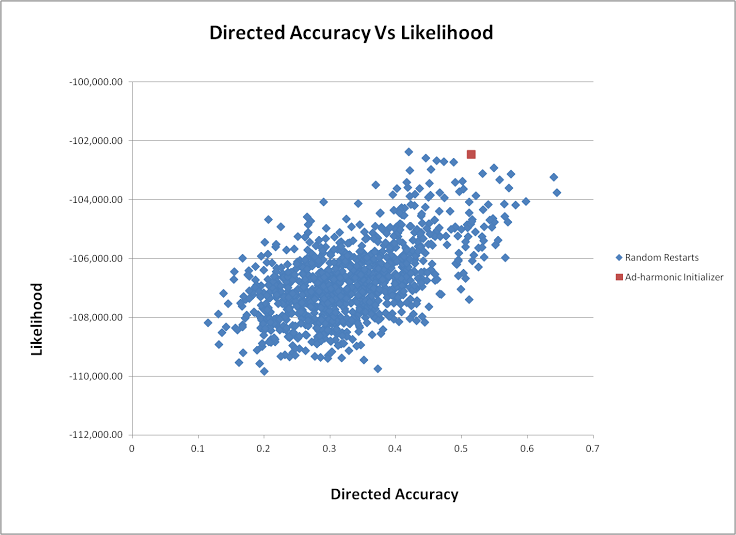
\includegraphics[width=90mm]{images/directed_accuracy.png}
\caption{Directed accuracy vs likelihood}
\label{overflow}
\end{figure}

\begin{figure}
\centering
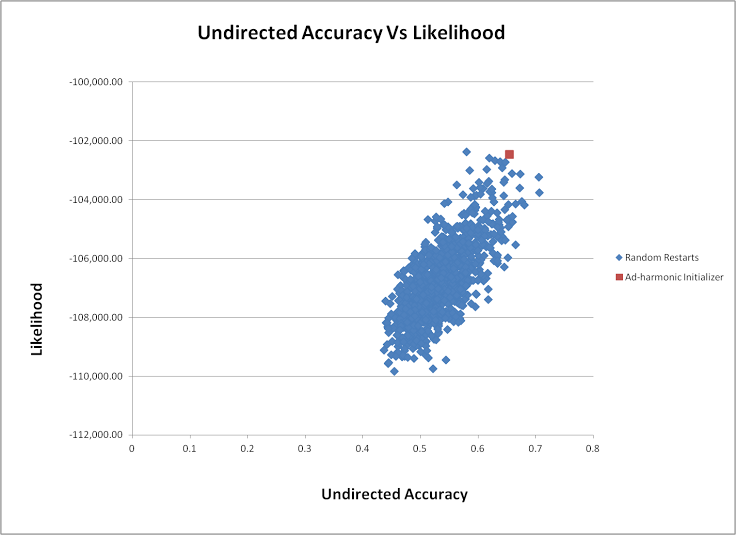
\includegraphics[width=90mm]{images/undirected_accuracy.png}
\caption{Undirected accuracy vs likelihood}
\label{overflow}
\end{figure}


\begin{table}[htbp]
\onehalfspacing
\begin{center}
\begin{tabular}{|l|c|r|}
\hline
\textbf{Characteristic} & \textbf{Ad-harmonic Initializer} & \textbf{Random Initializer}\\
\hline
Undirected accuracy &  65.5   &    70.56 (+5.06) \\
Directed accuracy &  51.5   &   55.59 (+4.09) \\
Likelihood &  -102,453.49   &  -102,375.79 (-77.7) \\
\hline
\end{tabular}
\end{center}
\caption{Comparing accuracies of Ad-harmonic and Random Initializer}
\end{table}


In order to see how the accuracy increases over the iterations, the EM was run for 60 iterations and the model was evaluated after every iteration. The directed accuracy after 1 iteration was 20.24\%. There is a steep increase until 30\% after which it is increasing gradually. The rate of increase after 35\% is very low. The average directed accuracy after 60 iterations is 36.18\%. In the case of undirected accuracy, there is a steep increase from 35\% to 49\% after which the rate of increase is considerably low. The average undirected accuracy after 60 iterations is 56.03\%.

\begin{figure}[!ht]
\centering
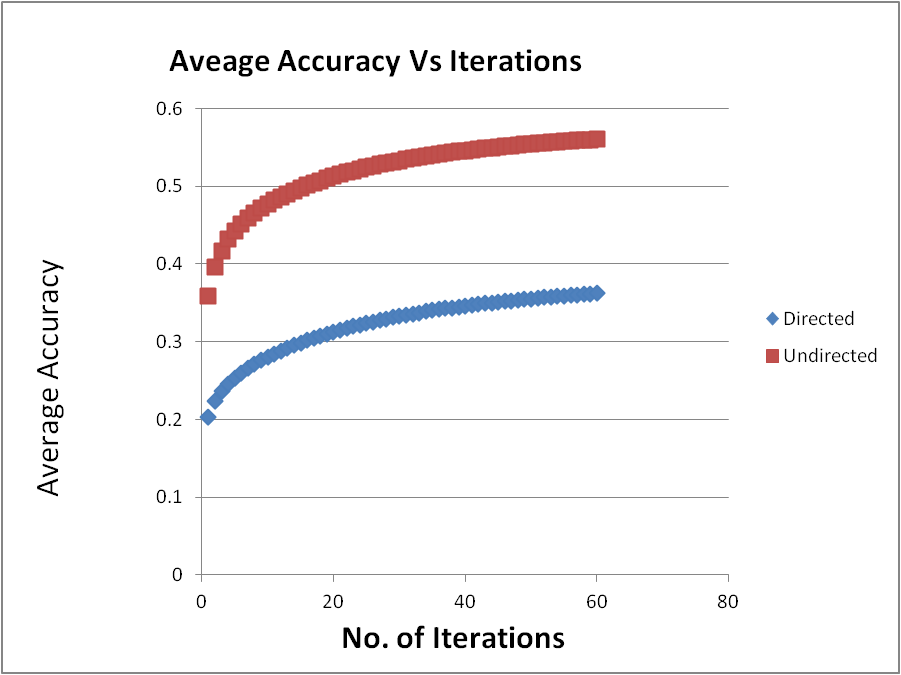
\includegraphics[width=90mm]{images/avg_accuracy.png}
\caption{Average accuracy per iteration}
\label{overflow}
\end{figure}

The average log-likelihood was computed by running the EM algorithm for 40 iterations. It was found that despite 40 iterations, the EM did not converge for any of the models. The likelihood after the first iteration was -198,707.45. It increased upto -103,271.23 at the end of 40 iterations. The slope decreased considerably after the 26th iteration and it was almost zero after the 35th iteration.

\begin{figure}[!ht]
\centering
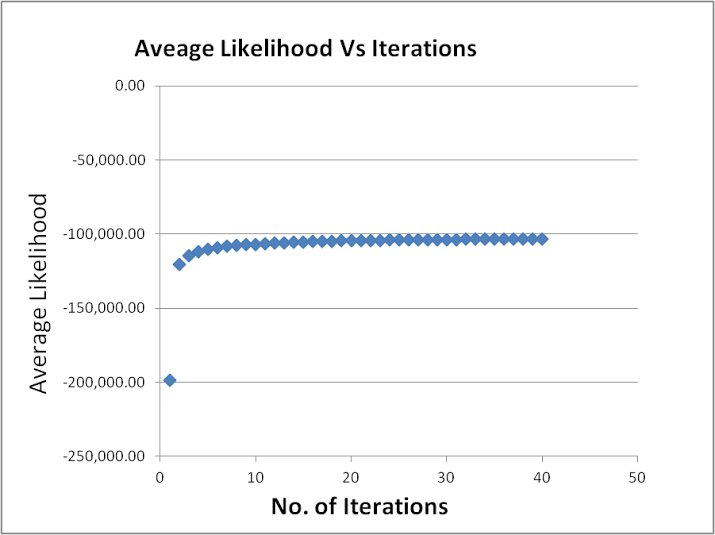
\includegraphics[width=90mm]{images/avg_likelihood.png}
\caption{Average likelihood per iteration}
\label{overflow}
\end{figure}


\section{Future Work}

Currently it takes 180 minutes to run EM for 60 iterations with 40 random restarts. For $k$ random restarts, the current implementation necessitates mainintaning all the $k$ multinomials in memory. After building a hypergraph for each sentence, the counts for every one of these multinomials is updated. Thus, the time taken to build the model is directly proportional to the number of multinomials, $k$. In order to scale to a million random restarts, the time taken to build the model must be independent of the number of random restarts. To achieve this, we intend to update the counts of each of the multinomials parallely.

%\bibliographystyle{apalike}
\bibliographystyle{plainnat}
\bibliography{thesis}

\end{document}
